\documentclass[letterpaper,openany,oneside,twocolumn]{book}

\newcommand{\PATH}{../../}

\usepackage{\PATH templates/utilities/m4rz-fonts}
\usepackage{\PATH templates/utilities/m4rz-colors}

\usepackage[justified]{\PATH templates/template_dnd/dnd}

\usepackage{\PATH templates/template_character-sheet/character-sheet-stylesheet}
\usepackage{\PATH templates/template_magic-item/magic-items-commands}

\setlength\oddsidemargin{\dimexpr(\paperwidth-\textwidth)/2 - 1in\relax}
\setlength\evensidemargin{\oddsidemargin}

% Headline
\CharacterName{Alistair Hellstrum}

\Class{Bard}
\MultiClassMainLevel{4}
\MultiClass{Warlock}
\Level{5}
\Background{Courtier}
\PlayerName{M4RZ}
\Race{Tiefling}
\Alignment{Chaotic Good (Neutral)}
\XP{}

% Ability scores (correct scores, no modifiers are automatically applied)
% Modifiers, Saving Throws and Skills are calculated automatically
\StrengthRolledScore{10}
\DexterityRolledScore{13}
\ConstitutionRolledScore{10}
\IntelligenceRolledScore{13}
\WisdomRolledScore{12}
\CharismaRolledScore{15}

\StrengthScoreBonus{0}
\DexterityScoreBonus{1} % ASI +1
\ConstitutionScoreBonus{0}
\IntelligenceScoreBonus{1} % Tiefling-Race +1
\WisdomScoreBonus{0}
\CharismaScoreBonus{3} % Tiefling-Race +2, ASI +1

\calculateAbilityScores{}

% Proficiencies (Proficient = 'P', Expertise = 'E', otherwise = '')
\StrengthProficiency{}
\DexterityProficiency{P}
\ConstitutionProficiency{}
\IntelligenceProficiency{}
\WisdomProficiency{}
\CharismaProficiency{P}

\AcrobaticsProficiency{P}
\AnimalHandlingProficiency{}
\ArcanaProficiency{P}
\AthleticsProficiency{}
\DeceptionProficiency{E}
\HistoryProficiency{P}
\InsightProficiency{P}
\IntimidationProficiency{P}
\InvestigationProficiency{}
\MedicineProficiency{}
\NatureProficiency{}
\PerceptionProficiency{}
\PerformanceProficiency{E}
\PersuasionProficiency{E} % Courtier Background
\ReligionProficiency{}
\SleightOfHandProficiency{}
\StealthProficiency{}
\SurvivalProficiency{}

% ABILITY MODIFIERS BONUS
\StrengthModifierBonus{0}
\DexterityModifierBonus{0}
\ConstitutionModifierBonus{0}
\IntelligenceModifierBonus{0}
\WisdomModifierBonus{0}
\CharismaModifierBonus{1} % Enchanted Locket of Lysandra Stage I

\Inspiration{}
\Proficiency{+3}
\PassivePerceptionModifier{1}

% Armor Class is not automatically calculated
\ArmorClass{\intcalcAdd{11}{\calculateModifier{\DexterityScoreValue}}}
\InitiativeModifier{0}
\Speed{30ft}
\MaxHitPointsRolled{34} % Without Constitution Bonus, is added automatically
\CurrentHitPoints{}
\TemporaryHitPoints{}
\HitDice{d8}
\HitDiceSpent{0}

\CP{}
\SP{}
\EP{}
\GP{355}
\PP{}

% Weapon Arsenal
\addWeaponStatistic{Rapier}{AlistairHellstrum}{DEX}{P}{0}{1d8 p}
\addWeaponStatistic{Dagger}{AlistairHellstrum}{DEX}{P}{0}{1d4 p}
\addWeaponStatistic{Unarmed Strike}{AlistairHellstrum}{STR}{P}{0}{\intcalcAdd{1}{\calculateModifier{\StrengthScoreValue}} b}

\AttacksAdditional{
	\textbf{Weapons:}
	\begin{itemize}
		\item Rapier
		\item Dagger
	\end{itemize}
	\textbf{Psychic Blades} (\DndDice{2d6})\\
	\textbf{Eldritch Blast} (2 Beams,\calculateModifier{\CharismaScoreValue} damage)\\
	\textbf{Mind Sliver} (\DndDice{2d6})\\
	\textbf{Vicious Mockery} (\DndDice{2d4})\\
	\textbf{Fey Presence}
}

\OtherProficienciesLanguages{
\textbf{Languages:}\\Common, Infernal\\
\textbf{Armor:}\\Light Armor\\
\textbf{Weapons:}\\Simple Weapons, Hand Crossbows, Longswords, Rapiers, Shortswords\\
\textbf{Tools:}\\Bagpipe, Lure, Violin
}

\Equipment{
	\textbf{Fochlucan Bandore}, \textbf{Eliwick's blank sheet of paper}, \textbf{Ring of the Feywild Dryads}, \textbf{Enchanted Locket of Lysandra} \\
	Leather Armor\\
	1 ruby (medium), 1 sapphire (medium), 2 silvered pine cones, Beetle in a Sweet, Cat Eye, Candy
}
\Clutter{
	 a backpack, a bedroll, 2 costumes, 5 candles, 5 days of ration, a waterskin, a disguise kit
}

\PersonalityTraits{
	\textbf{Charismatic:} Alistair possesses a natural charm and magnetic personality that draws people to him. He has a way with words and a captivating presence that allows him to easily connect with others.
}

\Ideals{
	\textbf{Musical Legacy:} Alistair is deeply connected to his musical heritage. He carries the weight of his family's musical lineage and strives to honor their legacy through his performances.
}

\Bonds{
	\textbf{Freedom of Expression:} Alistair believes in the power of artistic expression as a means of personal and societal liberation.
}

\Flaws{
	\textbf{Impulsive:} Alistair's passionate nature sometimes leads him to act on impulse, without considering the potential consequences.
}

\FeaturesTraits{
\textbf{Tiefling Traits}
\begin{itemize}
	\item Darkvision
	\item Hellish Resistance
	\item Infernal Legacy
\end{itemize}
\textbf{Court Functionary}
\begin{itemize}
	\item Charismatic Presence
	\item Eloquent Performer
\end{itemize}
\textbf{Eldritch Adept}
\begin{itemize}
	\item Agonizing Blast
\end{itemize}
\textbf{Bard}
\begin{itemize}
	\item Bardic Inspiration
	\item Jack-of-All-Trades
	\item Song of Rest
	\item Bard College of Whispers
	\begin{itemize}
		\item Psychic Blades
		\item Words of Terror
	\end{itemize}
\end{itemize}
\textbf{Warlock}
\begin{itemize}
	\item Otherworldly Patron (The Archfey)
	\item Eldritch Invocations
	\begin{itemize}
		\item Agonizing Blast
	\end{itemize}
\end{itemize}
\textbf{Charm of the Monarch}\\
\textbf{Compulsion (Locket)}
\begin{itemize}
	\item CHA-Checks +1
\end{itemize}
}

% Appearance

\Age{34}
\Height{6'1}
\Weight{150lbs}
\Eyes{Golden-Amber}
\Skin{Burgundy}
\Hair{Black}

% background

\CharacterAppearance{}{
	\hspace*{-1.5em}\begin{tabular}{p{90pt}p{75pt}}
		\begin{tabular}{p{90pt}}\vspace*{-2em}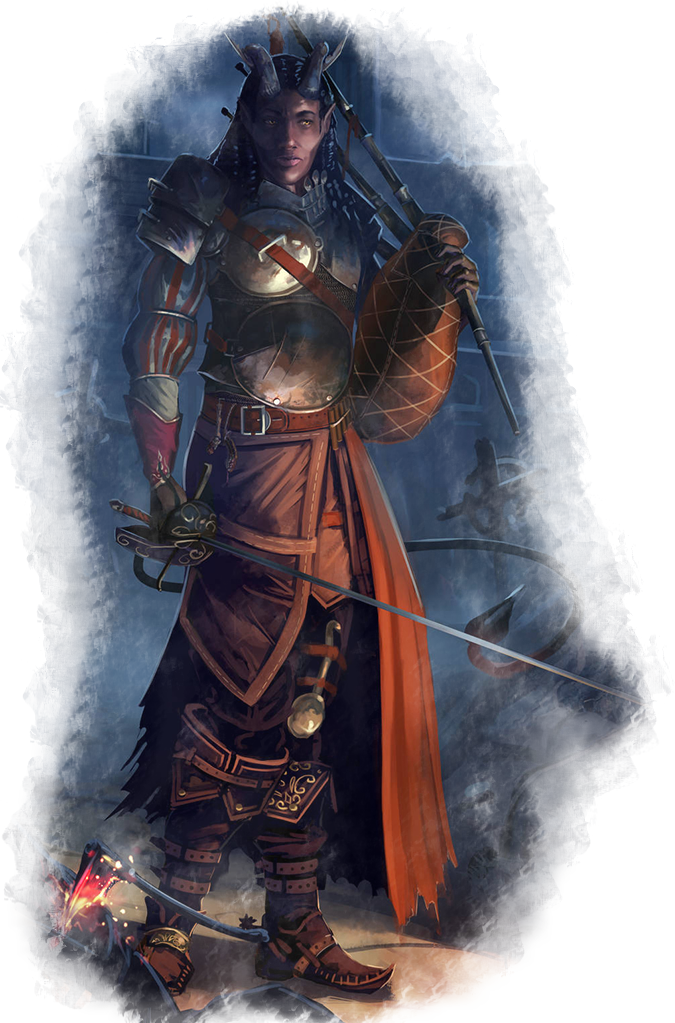
\includegraphics[width=100pt, height=140pt, keepaspectratio]{images/Alistair_appearance.png}\end{tabular}
		&
		\hspace*{-0.95em}\begin{tabular}{p{75pt}}Alistair Hellstrum stands at an average height with a lean and agile build. His skin has a rich, deep burgundy hue, a testament to his infernal heritage as a Tiefling. His eyes are a striking shade of golden ~~~~~~~~~\end{tabular}
	\end{tabular}\\\vspace*{-1.6em}\hfill\\
	amber, shimmering with a mischievous glint and an air of confidence. Alistair's dark, wavy hair cascades down to his shoulders, accentuating his charismatic and somewhat untamed demeanor.
}{}{}{}
\AdditionalFeaturesAndTraits{
	Alistair is not only a skilled musician but also a versatile performer. He excels in various forms of artistic expression, including acting, storytelling, and dancing. His performances are captivating and immersive, captivating audiences with their richness and variety.\\
	Alistair has a talent for languages and has devoted time to learning and mastering multiple tongues. In addition to Common and Infernal, he may be fluent in Elvish, Dwarvish, or other languages he has encountered during his travels. This linguistic ability allows him to connect with diverse cultures and communicate effectively with a wide range of individuals.\\
	Alistair has developed impressive negotiation skills over the years. He can find common ground and resolve conflicts through diplomacy and tact. His silver tongue, combined with his ability to read people, gives him an advantage in navigating delicate social and political situations.\\
	Alistair has a keen interest in the arcane arts and has studied magical theory and lore. Though not a full-fledged spellcaster, he possesses a solid understanding of magic and can identify magical items, comprehend magical writings, and recognize spells being cast.
}
\Characterbackground{
	Alistair Hellstrum's journey began in a bustling port city, where he was born to a humble family. From a young age, Alistair showed a natural inclination towards music and performance. He would often spend his days enchanting passersby with his melodious voice and captivating tunes, earning him a few copper coins to help support his family.
	
	However, life in the city was not without its challenges. Alistair's Tiefling heritage made him a target of prejudice and mistrust from some of the city's residents. Determined to rise above the discrimination, Alistair honed his talents, pouring his heart and soul into his music. His enchanting performances became a beacon of hope and inspiration for others who faced similar struggles.
	
	With his silver tongue, mesmerizing melodies, and unwavering spirit, Alistair Hellstrum, the Tiefling Bard, carries the torch of hope and harmony wherever his journey takes him.
}
\Treasure{
	\textbf{1. Ancient Manuscript:} Alistair possesses a weathered and meticulously preserved manuscript filled with ancient songs, stories, and forgotten lore. The pages are yellowed with age, and delicate illustrations adorn its margins. This precious relic is a treasure trove of inspiration, containing forgotten melodies, tales of legendary heroes, and cryptic clues that hint at hidden places of power.\\
	\textbf{2. Curious Relic (The Enchanted Locket of Lysandra):} Alistair possesses a peculiar relic, a seemingly ordinary, unadorned silver locket on a delicate chain. To the casual observer, it looks like an ordinary piece of jewelry with no special significance. However, upon closer inspection, faint, ever-shifting patterns of light dance across its surface, hinting at its magical nature.\\
	Unbeknownst to Alistair it kindles an insatiable fascination with the Fewild, which becomes stronger the more he interacts with the Feywild and its creatures.
}
\AlliesAndOrganizations{
	Most folk are happy to welcome a bard into their midst. Bards of the College of Whispers use this to their advantage. They appear to be like any other bard, sharing news, singing songs, and telling tales to the audiences they gather. In truth, the College of Whispers teaches its students that they are wolves among sheep. These bards use their knowledge and magic to uncover secrets and turn them against others through extortion and threats.

	Many other bards hate the College of Whispers, viewing it as a parasite that uses the bards' reputation to acquire wealth and power. For this reason, these bards rarely\linebreak
}{
	reveal their true nature unless they must. They typically claim to follow some other college, or keep their true nature secret in order to better infiltrate and exploit royal courts and other settings of power.
}
\OrganizationName{Bard College of Whispers}
\OrganizationSymbol{images/Bard_College_of_Lore.png}

% Magic

\SpellcastingClass{Bard/Warlock}
\SpellcastingAbility{CHA} % STR, DEX, CON, INT, WIS, CHA
\SpellSaveDCModifier{\CharismaModifierBonusValue} % any modifier that isn't contained in "8 + Ability Modifier + Proficiency Bonus"
\SpellAttackModifier{\CharismaModifierBonusValue} % any modifier that isn't contained in "Ability Modifier + Proficiency Bonus"


\CantripSlotA{Eldritch Blast (V, S)}
\CantripSlotB{Mage Hand (V, S)}
\CantripSlotC{Mind Sliver (V)}
\CantripSlotD{Prestidigitation (V, S)}
\CantripSlotE{Vicious Mockery (V)}

\CantripSlotG{Shillelagh (V, S, M) (once per day)}
\CantripSlotH{Thaumaturgy (V) (once per day)}

\FirstLevelSpellSlotsTotal{5} % 4 Bard + 1 Warlock
\FirstLevelSpellSlotA{Armor of Agathys (V, S, M)}
\FirstLevelSpellSlotB{Charm Person (V, S)}
\FirstLevelSpellSlotC{Dissonant Whispers (V)}
\FirstLevelSpellSlotD{Feather Fall (V, M)}
\FirstLevelSpellSlotE{Healing Word (V)}
\FirstLevelSpellSlotF{Hex (V, S, M)}

\FirstLevelSpellSlotH{Once per Day:}
\FirstLevelSpellSlotI{Entangle (V, S)}
\FirstLevelSpellSlotJ{Faerie Fire (V)}
\FirstLevelSpellSlotK{Hellish Rebuke (V, S)}
\FirstLevelSpellSlotL{Protection from Evil and Good (V, S)}
\FirstLevelSpellSlotM{Speak With Animals (V, S)}

\SecondLevelSpellSlotsTotal{3}
\SecondLevelSpellSlotA{Invisibility (V, S, M)}
\SecondLevelSpellSlotB{Shatter (V, S, M)}
\SecondLevelSpellSlotC{Suggestion (V, M)}

\SecondLevelSpellSlotJ{Once per Day:}
\SecondLevelSpellSlotK{Darkness (V, M)}
\SecondLevelSpellSlotL{Invisibility (V, S, M)}
\SecondLevelSpellSlotM{Levitate (V, S, M)}

\ThirdLevelSpellSlotK{Once per Day:}
\ThirdLevelSpellSlotL{Fly (V, S, M)}
\ThirdLevelSpellSlotM{Meld into Trees (V, S)}

\begin{document}

\newgeometry{left=0cm,right=0cm,top=0cm,bottom=0cm}
\onecolumn


% CHARACTER PAGE
\rendercharactersheet

% BACKSTORY PAGE
\renderbackgroundsheet

% SPELLCASTING PAGE
\renderspellsheet


\restoregeometry
\twocolumn

\chapter*{Recent Backstory}

{\noindent \entryfont \DndDropCapLine{A}listair, a talented and curious Tiefling bard, led a life of modest contentment. He wandered through towns and villages, sharing his songs and stories with eager audiences, unaware of the mystical wonders that lay beyond the realm of his knowledge. Little did he know that his fate was about to take an enchanting turn. He had performed for kings and peasants alike, honing his bardic talents and captivating audiences with stories of far-off lands.

One fateful day, while traversing a dense forest, Alistair's path led him to a secluded glade untouched by time. There, nestled amidst a bed of vibrant wildflowers, lay a silver locket, emitting a faint, otherworldly glow. Intrigued, he picked it up, feeling an immediate connection - a pulse of magic that resonated deep within his being. Alistair was slowly but steadily overcome by a rush of inexplicable emotions, as if the locket had awakened a part of him he never knew existed.

As the locket's magic flowed through him, Alistair's perception of the world began to shift. Vivid dreams of the Feywild's ethereal landscapes filled his nights, drawing him into a realm of enchantment and whimsy. The locket's melodies echoed in his mind, its whispers of the Feywild's beauty and mystery becoming a siren's call that he could not ignore.\\

\paragraph*{A Peculiar Encounter} During his newfound journey of discovery, Alistair's path crossed with that of a peculiar cleric named Alaric Kain. Known not only for his devotion to his deity but also for his insatiable cleptomania, Alaric was a charismatic individual with a penchant for getting into and especially out of trouble.

Their meeting was far from cordial. One serene afternoon, Alistair discovered Alaric attempting to pilfer a trinket from his belongings. Swift as a breeze, Alistair caught the cleric in the act, their gazes locking in a tense standoff. The air crackled with tension as Alistair demanded an explanation for the attempted theft. Alaric, undeterred, smirked and admitted his intent, claiming that he had sensed the locket's magical energy and was driven to understand its potential.

Despite the initial confrontation, Alistair's curiosity led him to strike an unlikely alliance with Alaric. Recognizing that they both harbored a burning desire to reach the Feywild, they decided to set aside their differences. While Alistair was wary of Alaric's tendencies, the shared goal of uncovering the mysteries of the Feywild provided a common purpose that bound them together.

As Alistair and Alaric journeyed together, their dynamic was a mix of camaraderie and tension. Alistair held the locket close, his attachment unbreakable, while Alaric's kleptomania occasionally caused friction. Yet, the shared goal of reaching the Feywild acted as a beacon, guiding them through challenges and obstacles.

\eject

\paragraph*{Enchanting Carnival} Their path eventually led them to a new destination - the Witchlight Carnival. The sound of music and laughter filled the air as they approached, signaling the arrival of the carnival. For Alistair and Alaric, this was not just another carnival - it was a stepping stone on their journey to the Feywild, a realm of dreams and mysteries waiting to be unveiled.

As they entered the carnival's enchanting realm, they were both acutely aware that their alliance held the potential to lead them to the heart of the Feywild itself. The locket's whispering enchantment was a constant reminder of the destiny that awaited them - one of discovery, danger, and the intertwining of their fates.

And so, under the starlit sky, Alistair and Alaric explored their surroundings, united by the allure of the Feywild and the shared pursuit of the mysteries behind the Enchanted Locket of Lysandra. At the Witchlight Carnival their journey was about to take an unexpected turn, where the lines between reality and enchantment would blur, and the whimsy of the Feywild would guide them toward their destiny.
}

\chapter*{A Dark, Mischievous Pact}
\noindent Alistair Hellstrum's transformation into a Warlock of the Archfey was profoundly shaped by a devastating loss and near-death experience during a harrowing encounter with Granny Nightshade. This critical moment unfolded within her lair, ingeniously crafted inside a massive fallen tree trunk, nestled in a peculiar village inhabited by her goblin and tin soldier entourage.

During this encounter, Granny Nightshade, a formidable fey-witch known for her cruelty and magical prowess, revealed her terrifying true form as a young red dragon, setting her surroundings ablaze and overwhelming Alistair and his companions. In the chaos, Alistair was struck down, and his life teetered on the brink of the abyss.

Miraculously, his companions managed to revive him from the edge of death. However, Alistair's consciousness clung to a singular, vivid memory - feeling the enchanted locket he wore, known as the Locket of Lysandra, pulling him back from the precipice of mortality. This locket, imbued with a mysterious power, seemed to guide him to safety, or so he believed.

As Alistair recovered from his injuries, the influence of the locket grew exponentially. Its whispers became louder, and visions of Lysandra, an enigmatic figure from the Feywild, began to haunt his dreams. Night after night, Lysandra visited him in these dreams, her voice both honeyed and tinged with darkness, promising him untold power and a destiny intertwined with her own.

Driven by a mixture of curiosity, longing for power, and a desire to transcend his mortal limitations, Alistair was drawn deeper into the enigmatic allure of the Feywild. He ultimately made a fateful decision to forge a pact with Lysandra. This pact bound his fate to hers, sealing his transformation with each promise whispered in the shadows of the Feywild.

With the power of the Archfey coursing through his veins, Alistair's persona began to change. His once jovial demeanor waned, his laughter turned hollow, and his smiles were tinged with shadows. His music adopted a darker tone, reflecting the deep and sometimes macabre influence of his new patron.

As days passed, Alistair found himself drifting further from his previous path, his morals eroding under the weight of his newfound abilities. The mischievous and sometimes malevolent influence of Lysandra twisted his perceptions, leading him down a morally ambiguous path where the distinction between right and wrong blurred into obscurity. This marked the beginning of Alistair's journey as a warlock, forever changed by the locket's pull and the shadowy promises of the Feywild.
\vspace*{-1.8\fontdimen6\font}\begin{center}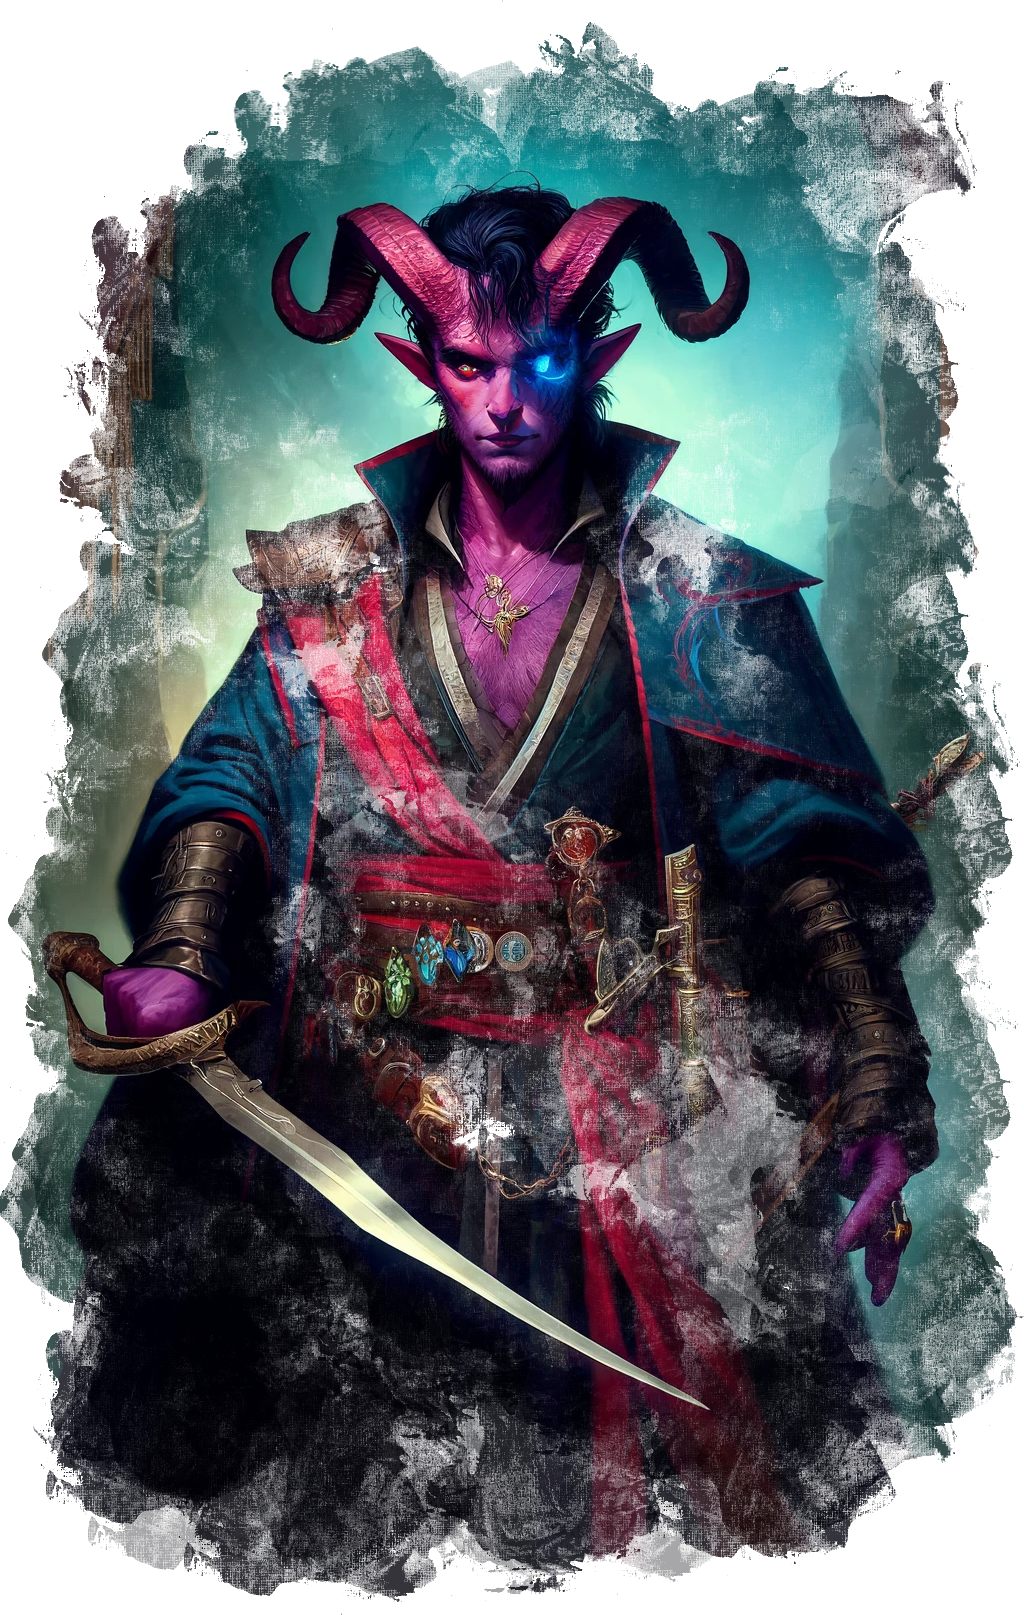
\includegraphics[scale=0.222]{images/Alistair_Warlock_Appearance.png}\end{center}\vspace*{-4.8\fontdimen6\font}\hfill\\
\subsection*{Lingering Injury}
Due to the severe injuries sustained during his harrowing battle with Granny Nightshade, Alistair Hellstrum now bears a grim reminder of his near-fatal defeat. He has lost his left eye, a consequence that continually affects his abilities. The hollow socket, from which his eye once keenly observed the world, now emits faint weaves of magic, swirling with dark, eerie energies that enhance his new, malevolent appearance. This constant flow of arcane energy not only marks his visage with an unsettling aura but also impairs his depth perception and accuracy. As a result, Alistair suffers disadvantages on Wisdom (Perception) checks, struggling to fully grasp his surroundings, as well as on ranged weapon attacks, where his depth perception falters significantly. This lingering injury is a stark testament to the dangers he has faced and the dark path he now walks as a warlock.

\chapter*{Features, Magic Items and Spells}

\section*{Tiefling Traits}
\subsection*{Darkvision}
Thanks to your infernal heritage, you have superior vision in dark and dim conditions. You can see in dim light within 60 feet of you as if it were bright light, and in darkness as if it were dim light. You can't discern color in darkness, only shades of gray.
\subsection*{Hellish Resistance}
You have resistance to fire damage.
\subsection*{Infernal Legacy}
You know the Thaumaturgy cantrip. Once you reach 3rd level, you can cast the Hellish Rebuke spell once as a 2nd-level spell. Once you reach 5th level, you can also cast the Darkness spell once. You must finish a long rest to cast these spells again with this trait. Charisma is your spellcasting ability for these spells.

\section*{Court Functionary}
Your knowledge of how bureaucracies function lets you gain access to the records and inner workings of any noble court or government you encounter. You know who the movers and shakers are, whom to go to for the favors you seek, and what the current intrigues of interest in the group are.
\subsection*{Charismatic Presence}
You gain proficiency in the Persuasion skill if you don't already have it. If you already have proficiency in Persuasion, you gain expertise in that skill, doubling your proficiency bonus for ability checks made with it.
\subsection*{Eloquent Performer}
When you use the Performance skill to entertain, inspire, or captivate an audience, your performance is exceptionally compelling. You have advantage on Performance checks made to impress or engage a crowd.

\section*{Eldritch Adept}
\textbf{Agonizing Blast}\\
Studying occult lore, you learn one Eldritch Invocation option of your choice from the warlock class. Your spellcasting ability for the invocation is Intelligence, Wisdom, or Charisma (choose when you select this feat). If the invocation has a prerequisite of any kind, you can choose that invocation only if you’re a warlock who meets the prerequisite.

Whenever you gain a level, you can replace the invocation with another one from the warlock class.

\section*{Bard Traits}
\subsection*{Bardic Inspiration}
You can inspire others through stirring words or music. To do so, you use a bonus action on your turn to choose one creature other than yourself within 60 feet of you who can hear you. That creature gains one Bardic Inspiration die, a d6.

Once within the next 10 minutes, the creature can roll the die and add the number rolled to one ability check, attack roll, or saving throw it makes. The creature can wait until after it rolls the d20 before deciding to use the Bardic Inspiration die, but must decide before the DM says whether the roll succeeds or fails. Once the Bardic Inspiration die is rolled, it is lost. A creature can have only one Bardic Inspiration die at a time.

You can use this feature a number of times equal to your Charisma modifier (a minimum of once). You regain any expended uses when you finish a long rest.

Your Bardic Inspiration die changes when you reach certain levels in this class. The die becomes a d8 at 5th level, a d10 at 10th level, and a d12 at 15th level.

(\textbf{Usages: \intcalcAdd{0}{\calculateModifier{\CharismaScoreValue}}})
\subsection*{Jack-of-All-Trades}
Starting at 2nd level, you can add half your proficiency bonus, rounded down, to any ability check you make that doesn't already include your proficiency bonus.
\subsection*{Song of Rest}
Beginning at 2nd level, you can use soothing music or oration to help revitalize your wounded allies during a short rest. If you or any friendly creatures who can hear your performance regain hit points at the end of the short rest by spending one or more Hit Dice, each of those creatures regains an extra 1d6 hit points.

The extra Hit Points increase when you reach certain levels in this class: to 1d8 at 9th level, to 1d10 at 13th level, and to 1d12 at 17th level.
\subsection*{Bard College of Whispers}
\subsubsection*{Psychic Blades}
When you join the College of Whispers at 3rd level, you gain the ability to make your weapon attacks magically toxic to a creature's mind.

When you hit a creature with a weapon attack, you can expend one use of your Bardic Inspiration to deal an additional 2d6 psychic damage to that target. You can do so only once per round on your turn.

The psychic damage increases when you reach certain levels in this class, increasing to 3d6 at 5th level, 5d6 at 10th level, and 8d6 at 15th level.

\subsubsection*{Words of Terror}
At 3rd level, you learn to infuse innocent-seeming words with an insidious magic that can inspire terror.

If you speak to a humanoid alone for at least 1 minute, you can attempt to seed paranoia and fear into its mind. At the end of the conversation, the target must succeed on a Wisdom saving throw against your spell save DC or be frightened of you or another creature of your choice. The target is frightened in this way for 1 hour, until it is attacked or damaged, or until it witnesses its allies being attacked or damaged.

If the target succeeds on its saving throw, the target has no hint that you tried to frighten it.

Once you use this feature, you can't use it again until you finish a short rest or long rest.

\section*{Warlock Traits}
\subsection*{Otherworldly Patron}
\subsubsection*{The Archfey}
Your patron is a lord or lady of the fey, a creature of legend who holds secrets that were forgotten before the mortal races were born. This being's motivations are often inscrutable, and sometimes whimsical, and might involve a striving for greater magical power or the settling of age-old grudges. Beings of this sort include the Prince of Frost; the Queen of Air and Darkness, ruler of the Gloaming Court; Titania of the Summer Court; her consort Oberon, the Green Lord; Hyrsam, the Prince of Fools; and ancient hags.
\subsubsection*{Expended Spell List}
The Archfey lets you choose from an expanded list of spells when you learn a warlock spell. The following spells are added to the warlock spell list for you.
\begin{DndTable}[header=Archfey Expanded Spells]{llX}
			& \textbf{Spell Level}  	&\textbf{Spells}						\\
$\bullet$	& 1st						&Faerie Fire, Sleep						\\
			& 2nd						&Calm Emotions, Phantasmal Force		\\
			& 3rd						&Blink, Plant Growth					\\
			& 4th						&Dominate Beast, Greater Invisibility	\\
			& 5th						&Dominate Person, Seeming				\\
\end{DndTable}
\subsubsection*{Fey Presence}
Starting at 1st level, your patron bestows upon you the ability to project the beguiling and fearsome presence of the fey. As an action, you can cause each creature in a 10-foot cube originating from you to make a Wisdom saving throw against your warlock spell save DC. The creatures that fail their saving throws are all charmed or frightened by you (your choice) until the end of your next turn.

Once you use this feature, you can't use it again until you finish a short or long rest.

\subsection*{Eldritch Invocations}
In your study of occult lore, you have unearthed Eldritch Invocations, fragments of forbidden knowledge that imbue you with an abiding magical ability.

At 2nd level, you gain two eldritch invocations of your choice. When you gain certain warlock levels, you gain additional invocations of your choice, as shown in the Invocations Known column of the Warlock table. A level prerequisite refers to your level in this class.

Additionally, when you gain a level in this class, you can choose one of the invocations you know and replace it with another invocation that you could learn at that level.
\subsubsection*{Agonizing Blast}
When you cast eldritch blast, add your Charisma modifier to the damage it deals on a hit.

\section*{Other Traits}
\subsection*{Charm of the Monarch}
You can sprout a pair of beautiful butterfly wings, you gain flying speed equal to your walking speed, and you gain a +5 bonus on all Charisma-based ability checks. These effects last for 1 hour. After you use this charm two times, it vanishes from you.\\
\textbf{(Usages: 1)}

\section*{Spells}
\subsection*{Cantrip}

\DndSpellHeader
  {Eldritch Blast}
  {Evocation Cantrip}
  {1 Action}
  {120 feet}
  {V, S}
  {Instantaneous}
  
A beam of crackling energy streaks toward a creature within range. Make a ranged spell attack against the target. On a hit, the target takes 1d10 force damage.

\subparagraph*{At Higher Levels} The spell creates more than one beam when you reach higher levels: two beams at 5th level, three beams at 11th level, and four beams at 17th level. You can direct the beams at the same target or at different ones. Make a separate attack roll for each beam.

\DndSpellHeader
  {Mage Hand}
  {Cantrip Conjuration}
  {1 Action}
  {30 feet}
  {V, S}
  {1 Minute}
  
A spectral, floating hand appears at a point you choose within range. The hand lasts for the duration or until you dismiss it as an action. The hand vanishes if it is ever more than 30 feet away from you or if you cast this spell again.\\
You can use your action to control the hand. You can use the hand to manipulate an object, open an unlocked door or container, stow or retrieve an item from an open container, or pour the contents out of a vial. You can move the hand up to 30 feet each time you use it.\\
The hand can't attack, activate magic items, or carry more than 10 pounds.

\DndSpellHeader
  {Mind Sliver}
  {Enchantment Cantrip}
  {1 Action}
  {60 feet}
  {V}
  {1 Round}
  
You drive a disorienting spike of psychic energy into the mind of one creature you can see within range. The target must succeed on an Intelligence saving throw or take 1d6 psychic damage and subtract 1d4 from the next saving throw it makes before the end of your next turn.

\subparagraph*{At Higher Levels} This spell's damage increases by 1d6 when you reach certain levels: 5th level (2d6), 11th level (3d6), and 17th level (4d6).

\DndSpellHeader
  {Prestidigitation}
  {Cantrip Transmutation}
  {1 Action}
  {10 feet}
  {V, S}
  {up to 1 hour}

This spell is a minor magical trick that novice spellcasters use for practice. You create one of the following magical effects within range:\\
You create an instantaneous, harmless sensory effect, such as a shower of sparks, a puff of wind, faint musical notes, or an odd odor.\\
You instantaneously light or snuff out a candle, a torch, or a small campfire.\\
You instantaneously clean or soil an object no larger than 1 cubic foot.\\
You chill, warm, or flavor up to 1 cubic foot of nonliving material for 1 hour.\\
You make a color, a small mark, or a symbol appear on an object or a surface for 1 hour.\\
You create a nonmagical trinket or an illusory image that can fit in your hand and that lasts until the end of your next turn.\\
If you cast this spell multiple times, you can have up to three of its non-instantaneous effects active at a time, and you can dismiss such an effect as an action.

\DndSpellHeader
  {Shillelagh}
  {Cantrip Transmutation}
  {1 Bonus Action}
  {Touch}
  {V, S, M (Mistletoe, a shamrock leaf, and a club or quarterstaff)}
  {1 Minute}
  
The wood of a club or quarterstaff you are holding is imbued with nature's power. For the duration, you can use your spellcasting ability instead of Strength for the attack and damage rolls of melee attacks using that weapon, and the weapon's damage die becomes a d8. The weapon also becomes magical, if it isn't already. The spell ends if you cast it again or if you let go of the weapon.

\DndSpellHeader
  {Thaumaturgy}
  {Cantrip Transmutation}
  {1 Action}
  {30 feet}
  {V}
  {up to 1 minute}

You manifest a minor wonder, a sign of supernatural power create one of the following magical effects within range:\\
Your voice booms up to three times as loud as normal for 1 minute.\\
You cause flames to flicker, brighten, dim, or change color for 1 minute.\\
You cause harmless tremors in the ground for 1 minute.\\
You create an instantaneous sound that originates from a point of your choice within range, such as a rumble of thunder.\\
You instantaneously cause an unlocked door or window to fly open or slam shut.\\
You alter the appearance of your eyes for 1 minute.\\
If you cast this spell multiple times, you can have up to three of its effects active at a time, and you can dismiss such an effect as an action.\\

\DndSpellHeader
  {Vicious Mockery}
  {Cantrip Enchantment}
  {1 Action}
  {A creature you can see and that can hear you within range}
  {V}
  {Instantaneous}

You unleash a string of insults laced with subtle enchantments at a creature you can see within range. If the target can hear you (though it need not understand you), it must succeed on a Wisdom saving throw or take \DndDice{1d4} psychic damage and have disadvantage on the next attack roll it makes before the end of its next turn.

\subparagraph*{At Higher Levels} This spell's damage increases by 1d4 when you reach 5th level (2d4), 11th level (3d4), and 17th level (4d4).

\subsection*{Level 1}

\DndSpellHeader
  {Armor of Agathys}
  {1st Level Abjuration}
  {1 Action}
  {Self}
  {V, S, M (a cup of water)}
  {1 hour}
  
A protective magical force surrounds you, manifesting as a spectral frost that covers you and your gear. You gain 5 temporary hit points for the duration. If a creature hits you with a melee attack while you have these hit points, the creature takes 5 cold damage.

\subparagraph*{At Higher Levels} When you cast this spell using a spell slot of 2nd level or higher, both the temporary hit points and the cold damage increase by 5 for each slot.

\DndSpellHeader
  {Charm Person}
  {1st Level Enchantment}
  {1 Action}
  {30 feet}
  {V, S}
  {1 hour}

You attempt to charm a humanoid you can see within range. It must make a Wisdom saving throw, and does so with advantage if you or your companions are fighting it. If it fails the saving throw, it is charmed by you until the spell ends or until you or your companions do anything harmful to it. The charmed creature regards you as a friendly acquaintance. When the spell ends, the creature knows it was charmed by you.

\subparagraph*{At Higher Levels} When you cast this spell using a spell slot of 2nd level or higher, you can target one additional creature for each slot level above 1st. The creatures must be within 30 feet of each other when you target them.

\DndSpellHeader
  {Dissonant Whispers}
  {1st Level Enchantment}
  {1 Action}
  {60 feet}
  {V}
  {Instantaneous}

You whisper a discordant melody that only one creature of your choice within range can hear, wracking it with terrible pain. The target must make a Wisdom saving throw. On a failed save, it takes \DndDice{3d6} psychic damage and must immediately use its reaction, if available, to move as far as its speed allows away from you. The creature doesn't move into obviously dangerous ground, such as a fire or a pit. On a successful save, the target takes half as much damage and doesn't have to move away. A deafened creature automatically succeeds on the save.

\subparagraph*{At Higher Levels} When you cast this spell using a spell slot of 2nd level or higher, the damage increases by \DndDice{1d6} for each slot level above 1st.

\DndSpellHeader
  {Entangle}
  {1st Level Conjuration}
  {1 Action}
  {90 feet}
  {V, S}
  {Concentration, up to 1 Minute}
  
Grasping weeds and vines sprout from the ground in a 20-foot square starting from a point within range. For the duration, these plants turn the ground in the area into difficult terrain.\\
A creature in the area when you cast the spell must succeed on a Strength saving throw or be restrained by the entangling plants until the spell ends. A creature restrained by the plants can use its action to make a Strength check against your spell save DC. On a success, it frees itself.\\
When the spell ends, the conjured plants wilt away.

\DndSpellHeader
  {Faerie Fire}
  {1st-Level Evocation}
  {1 Action}
  {60 feet}
  {V}
  {Concentration, up to 1 Minute}

Each object in a 20-foot cube within range is outlined in blue, green, or violet light (your choice). Any creature in the area when the spell is cast is also outlined in light if it fails a Dexterity saving throw. For the duration, objects and affected creatures shed dim light in a 10-foot radius.

Any attack roll against an affected creature or object has advantage if the attacker can see it, and the affected creature or object can't benefit from being invisible.

\DndSpellHeader
  {Feather Fall}
  {1st-Level Transmutation}
  {1 Reaction, which you take when you or a creature within 60 feet of you falls}
  {60 feet}
  {V, M (A small feather or piece of down)}
  {1 Minute}

Choose up to five falling creatures within range. A falling creature's rate of descent slows to 60 feet per round until the spell ends. If the creature lands before the spell ends, it takes no falling damage and can land on its feet, and the spell ends for that creature.

\DndSpellHeader
  {Healing Word}
  {1st Level Evocation}
  {1 Bonus Action}
  {60 feet}
  {V}
  {Instantaneous}

A creature of your choice that you can see within range regains hit points equal to \DndDice{1d4} + your spellcasting ability modifier \textbf{(+\intcalcAdd{0}{\calculateModifier{\CharismaScoreValue}})}. This spell has no effect on undead or constructs.

\subparagraph*{At Higher Levels} When you cast this spell using a spell slot of 2nd level or higher, the Healing increases by \DndDice{1d4} for each slot level above 1st.

\DndSpellHeader
  {Hellish Rebuke}
  {1st Level Evocation}
  {1 Reaction, which you take in response to being damaged by a creature within 60 feet of you that you can see}
  {60 feet}
  {V, S}
  {Instantaneous}

You point your finger, and the creature that damaged you is momentarily surrounded by hellish flames. The creature must make a Dexterity saving throw. It takes \DndDice{2d10} fire damage on a failed save, or half as much damage on a successful one.

\subparagraph*{At Higher Levels} When you cast this spell using a spell slot of 2nd level or higher, the damage increases by \DndDice{1d10} for each slot level above 1st.

\DndSpellHeader
  {Hex}
  {1st Level Enchantment}
  {1 Bonus Action}
  {90 feet}
  {V, S, M (the petrified eye of a newt)}
  {Concentration, up to 1 Hour}
  
You place a curse on a creature that you can see within range. Until the spell ends, you deal an extra 1d6 necrotic damage to the target whenever you hit it with an attack. Also, choose one ability when you cast the spell. The target has disadvantage on ability checks made with the chosen ability.

If the target drops to 0 hit points before this spell ends, you can use a bonus action on a subsequent turn of yours to curse a new creature.

A Remove Curse cast on the target ends this spell early.

\subparagraph*{At Higher Levels} When you cast this spell using a spell slot of 3rd or 4th level, you can maintain your concentration on the spell for up to 8 hours. When you use a spell slot of 5th level or higher, you can maintain your concentration on the spell for up to 24 hours.

\DndSpellHeader
  {Protection from Evil and Good}
  {1st Level Abjuration}
  {1 Action}
  {Touch}
  {V, S, M (Holy water or powdered silver and iron, which the spell consumes)}
  {Concentration, up to 10 Minutes}
  
Until the spell ends, one willing creature you touch is protected against certain types of creatures: aberrations, celestials, elementals, fey, fiends, and undead.\\
The protection grants several benefits. Creatures of those types have disadvantage on attack rolls against the target. The target also can't be charmed, frightened, or possessed by them. If the target is already charmed, frightened, or possessed by such a creature, the target has advantage on any new saving throw against the relevant effect.

\DndSpellHeader
  {Speak with Animals}
  {1st Level Divination (Ritual)}
  {1 Action}
  {Self}
  {V, S}
  {10 Minutes}
  
You gain the ability to comprehend and verbally communicate with beasts for the duration. The knowledge and awareness of many beasts is limited by their intelligence, but at minimum, beasts can give you information about nearby locations and monsters, including whatever they can perceive or have perceived within the past day. You might be able to persuade a beast to perform a small favor for you, at the GM's discretion.

\subsection*{Level 2}

\DndSpellHeader
  {Darkness}
  {2nd Level Evocation}
  {1 Action}
  {60 feet}
  {V, M (Bat fur and a drop of pitch or piece of coal)}
  {Concentration, up to 10 Minutes}
  
Magical darkness spreads from a point you choose within range to fill a 15-foot-radius sphere for the duration. The darkness spreads around corners. A creature with darkvision can't see through this darkness, and nonmagical light can't illuminate it.

If the point you choose is on an object you are holding or one that isn't being worn or carried, the darkness emanates from the object and moves with it. Completely covering the source of the darkness with an opaque object, such as a bowl or a helm, blocks the darkness.

If any of this spell's area overlaps with an area of light created by a spell of 2nd level or lower, the spell that created the light is dispelled.

\DndSpellHeader
  {Invisibility}
  {2nd Level Illusion}
  {1 Action}
  {Touch}
  {V, S, M (An eyelash encased in gum arabic)}
  {Concentration, up to 1 Hour}
  
A creature you touch becomes invisible until the spell ends. Anything the target is wearing or carrying is invisible as long as it is on the target's person. The spell ends for a target that attacks or casts a spell.

\subparagraph*{At Higher Levels} When you cast this spell using a spell slot of 3rd level or higher, you can target one additional creature for each slot level above 2nd.

\DndSpellHeader
  {Levitate}
  {2nd Level Transmutation}
  {1 Action}
  {60 feet}
  {V, S, M (Either a small leather loop or a piece of golden wire bent into a cup shape with a long shank on one end)}
  {Concentration, up to 10 Minutes}
  
One creature or object of your choice that you can see within range rises vertically, up to 20 feet, and remains suspended there for the duration. The spell can levitate a target that weighs up to 500 pounds. An unwilling creature that succeeds on a Constitution saving throw is unaffected.\\
The target can move only by pushing or pulling against a fixed object or surface within reach (such as a wall or a ceiling), which allows it to move as if it were climbing. You can change the target's altitude by up to 20 feet in either direction on your turn. If you are the target, you can move up or down as part of your move. Otherwise, you can use your action to move the target, which must remain within the spell's range.\\
When the spell ends, the target floats gently to the ground if it is still aloft.

\DndSpellHeader
  {Shatter}
  {2nd Level Evocation}
  {1 Action}
  {60 feet}
  {V, S, M (A chip of mica)}
  {Instantaneous}

A sudden loud ringing noise, painfully intense, erupts from a point of your choice within range. Each creature in a 10-foot-radius sphere centered on that point must make a Constitution saving throw. A creature takes \DndDice{3d8} thunder damage on a failed save, or half as much damage on a successful one. A creature made of inorganic material such as stone, crystal, or metal has disadvantage on this saving throw. A nonmagical object that isn't being worn or carried also takes the damage if it's in the spell's area.

\subparagraph*{At Higher Levels} When you cast this spell using a spell slot of 3rd level or higher, the damage increases by \DndDice{1d8} for each slot level above 2nd.

\DndSpellHeader
  {Suggestion}
  {2nd Level Enchantment}
  {1 Action}
  {30 feet}
  {V, M (A snake's tongue and either a bit of honeycomb or a drop of sweet oil)}
  {Concentration, up to 8 Hours}

You suggest a course of activity (limited to a sentence or two) and magically influence a creature you can see within range that can hear and understand you. Creatures that can't be charmed are immune to this effect. The suggestion must be worded in such a manner as to make the course of action sound reasonable. Asking the creature to stab itself, throw itself onto a spear, immolate itself, or do some other obviously harmful act ends the spell.\\
The target must make a Wisdom saving throw. On a failed save, it pursues the course of action you described to the best of its ability. The suggested course of action can continue for the entire duration. If the suggested activity can be completed in a shorter time, the spell ends when the subject finishes what it was asked to do.\\
You can also specify conditions that will trigger a special activity during the duration. For example, you might suggest that a knight give her warhorse to the first beggar she meets. If the condition isn't met before the spell expires, the activity isn't performed.\\
If you or any of your companions damage the target, the spell ends.

\subsection*{Level 3}

\DndSpellHeader
  {Fly}
  {3rd Level Transmutation}
  {1 Action}
  {Touch}
  {V, S, M (A wing feather from any bird)}
  {Concentration, up to 10 Minutes}
  
You touch a willing creature. The target gains a flying speed of 60 feet for the duration. When the spell ends, the target falls if it is still aloft, unless it can stop the fall.

\subparagraph*{At Higher Levels} When you cast this spell using a spell slot of 4th level or higher, you can target one additional creature for each slot level above 3rd.

\DndSpellHeader
  {Meld into Trees}
  {3rd Level Transmutation (Ritual)}
  {1 Action}
  {Touch}
  {V, S}
  {8 Hours}
  
You step into a tree object or surface large enough to fully contain your body, melding yourself and all the equipment you carry with the tree for the duration. Using your movement, you step into the tree at a point you can touch. Nothing of your presence remains visible or otherwise detectable by nonmagical senses.
While merged with the tree, you can't see what occurs outside it, and any Wisdom (Perception) checks you make to hear sounds outside it are made with disadvantage. You remain aware of the passage of time and can cast spells on yourself while merged in the tree. You can use your movement to leave the tree where you entered it, which ends the spell. You otherwise can't move.
Minor physical damage to the tree doesn't harm you, but its partial destruction or a change in its shape (to the extent that you no longer fit within it) expels you and deals 6d6 bludgeoning damage to you. The tree's complete destruction (or transmutation into a different substance) expels you and deals 50 bludgeoning damage to you. If expelled, you fall prone in an unoccupied space closest to where you first entered.

\vfill\eject

\section*{Miscellaneous}
\subsection*{Attack and Damage Rolls}
\subsubsection*{Melee Weapons}
\paragraph*{Attack Roll}\hfill\\
\underline{\textit{Dagger (Finesse):}}\\
1d20 + DEX-Modifier + Proficiency Modifier\\
\indent Current Max: \intcalcAdd{20}{\intcalcAdd{\calculateModifier{\DexterityScoreValue}}{\ProficiencyValue}}
\\
\underline{\textit{Rapier (Finesse):}}\\
1d20 + DEX-Modifier + Proficiency Modifier\\
\indent Current Max: \intcalcAdd{20}{\intcalcAdd{\calculateModifier{\DexterityScoreValue}}{\ProficiencyValue}}
\paragraph*{Damage Roll}\hfill\\
\underline{\textit{Dagger (Finesse):}}\\
1d4 + DEX-Modifier\\
\indent Current Max: \intcalcAdd{4}{\calculateModifier{\DexterityScoreValue}}
\\
\underline{\textit{Rapier (Finesse):}}\\
1d8 + DEX-Modifier\\
\indent Current Max: \intcalcAdd{8}{\calculateModifier{\DexterityScoreValue}}
\subsubsection*{Special Attacks}
\paragraph*{Attack Roll}\hfill\\
\underline{\textit{Unarmed Strike:}}\\
1d20 + STR-Modifier + Proficiency Modifier\\
\indent Current Max: \intcalcAdd{20}{\intcalcAdd{\calculateModifier{\StrengthScoreValue}}{\ProficiencyValue}}
\paragraph*{Damage Roll}\hfill\\
\underline{\textit{Unarmed Strike:}}\\
1 + STR-Modifier\\
\indent Current Max: \intcalcAdd{1}{\calculateModifier{\StrengthScoreValue}}

% Magic Items
\ItemCategory{Instruments}
\ItemSubCategory{}
\ItemFolder{Fochlucan_Bandore}

\chapter*{Fochlucan Bandore}
\itemDescriptionAndImage{Wondrous item, instrument, uncommon (requires attunement by a bard)}{Fochlucan_Bandore.png}{10.25cm}\\

\textit{An instrument of the bards is an exquisite example of its kind, superior to an ordinary instrument in every way. Seven types of these instruments exist, each named after a legendary bard college.}

\section*{Appearance}
The "Fochlucan Bandore" is a mesmerizing musical instrument that beautifully merges the traditional forms of a bandore and a lute. It features an elegantly curved body, reminiscent of a bandore, but extends into a longer, slender neck characteristic of a lute, culminating in a distinctively crafted headstock. The instrument's surface is a canvas of intricate carvings and inlays, depicting mystical symbols and ancient runes, hinting at its magical origins. Its rich, warm wood tones are accentuated by a deep varnish, giving it an antique yet well-maintained appearance. Perhaps its most striking feature is its shimmering, light-like strings, adding a magical quality to its already ethereal aesthetic. This blend of artistic beauty, arcane significance, and ancient tradition renders the Fochlucan Bandore not just a musical instrument, but a remarkable piece of art and a mystical artifact, resonating with an aura of age-old lore and enchantment.

\section*{Arcane Challenge}
A creature that attempts to play the instrument without being attuned to it must succeed on a DC 15 Wisdom saving throw or take 2d4 psychic damage.

\section*{Charming Harmony}
You can play the instrument while casting a spell that causes any of its targets to be charmed on a failed saving throw, thereby imposing disadvantage on the save. This effect applies only if the spell has a somatic or a material component.

\section*{Spellcasting Ability}
You can use an action to play the instrument and cast one of its spells. Once the instrument has been used to cast a spell, it can't be used to cast that spell again until the next dawn. The spells use your spellcasting ability and spell save DC.
\subsection*{Standard Spells for Bard Instruments}
All instruments of the bards can be used to cast the following spells: Fly, Invisibility, Levitate, and Protection from Evil and Good.
\subsection*{Unique Spells of the Fochlucan Bandore}
In addition, the Fochlucan Bandore can be used to cast Entangle, Faerie Fire, Shillelagh, and Speak with Animals.
\ItemCategory{Jewellery}
\ItemSubCategory{Rings}
\ItemFolder{Ring_of_the_Feywild_Dryads}

\chapter*{Ring of the Feywild Dryads}
\itemDescriptionAndImage{Ring, uncommon (requires attunement)}{Ring_of_Meld_into_Trees.png}{11.25cm}
\section*{Appearance}
The "Ring of the Feywild Dryads" appears as a masterfully crafted piece of ancient magic and natural wonder. The band, formed from what seems to be twisted silver, mimics the intricate intertwining of tree branches, encircling the finger with a grace that speaks of the forest's deep and mystic ties. This silver has been textured to resemble bark, enhancing its bond with the trees it represents. At the heart of the ring, a large, captivating emerald sits prominently, its deep green hue glowing softly as if lit from within, symbolizing the life force of the forest and the essence of tree magic. Delicate Elvish runes, suggestive of enchantment and age-old secrets, are engraved along the band, hinting at the ring's ancient origins and its potent ability to connect the wearer with the natural world. This ring is not merely an accessory but a powerful artifact that embodies the spirit of the forest and the magic of melding with trees.
\vfill\eject
\section*{History}
The "Ring of the Feywild Dryads" is not merely a magical item; it is a relic of deep history and symbiotic power, born from the ancient alliance between the mortal realms and the feywilds. Crafted in an age long forgotten, under the boughs of the Eternal Forest in the heart of the feywilds, this ring was a gift from the dryads to the first of the Elven druids who walked the path between worlds.

The dryads, spirits of the trees, and guardians of the forest's deepest magics, sought to imbue this ring with the essence of their being and the forests they protect. Using silver that was mined from the sacred mountains surrounding the Eternal Forest and blessed by the light of the full moon, the ring was forged in the shape of intertwining branches, a symbol of life's complexity and interconnection. The centerpiece, a radiant emerald, was chosen for its resemblance to the heart of the forest - a gem that had captured the very essence of the feywild's verdant splendor.

Upon its creation, the Ring of the Feywild Dryads was bestowed upon an elf, chosen for their unwavering dedication to protecting the natural world. This elf, a druid of unparalleled connection to the earth's rhythms and cycles, became the first of many guardians who would wield the ring's power to merge with the trees, learning their secrets, and protecting the forests from those who would do them harm.

Over the centuries, the ring passed from one guardian to another, always finding its way to those who had proven themselves protectors of nature's sanctity. Each bearer left their mark on the ring, contributing to its legacy and the stories it holds within. Legends say that the ring still carries the whispers of the dryads and the echoes of the Eternal Forest, guiding its wearer not only to meld into trees but to understand the very language of the forest.

Today, the "Ring of the Feywild Dryads" remains a bridge between the mortal realms and the enchantments of the feywilds, a testament to the enduring alliance between the elves and the dryads. It is a reminder of the deep bonds that can form when different beings unite in a common cause, protecting the natural world and preserving its wonders for generations to come.
\section*{Magic}
While attuned to the ring, its wearer can cast the "Meld into Trees" spell once per long rest.
\ItemCategory{Jewellery}
\ItemSubCategory{Talisman}
\ItemFolder{Enchanted_Locket_of_Lysandra}

\chapter*{The Enchanted Locket of Lysandra}
\itemDescriptionAndImage{Locket, rare (requires attunement)}{Locket_of_Lysandra.png}{10cm}

\section*{Appearance}
The Enchanted Locket of Lysandra appears as a simple and unadorned silver locket on a delicate chain. To the casual observer, it looks like an ordinary piece of jewelry with no special significance. However, upon closer inspection, however, the true magic of the locket becomes apparent. Faint, ever-shifting patterns of light dance across its surface like playful fireflies on a warm summer night. These ethereal luminescent swirls seem to weave intricate stories, their fleeting forms conjuring images of blooming wildflowers, starlit skies, and the elusive spirits of the Feywild. Each flicker of light holds a hint of forgotten tales, a connection to a realm of dreams that exists just beyond the veil of perception.

Adding to the intrigue, the locket possesses a set of minuscule, intricately wrought hinges that are barely discernible to the naked eye. These hinges, delicate as the gossamer wings of a butterfly, are an enigma in themselves, for they hint at the locket's potential to open and reveal its secrets. Yet, despite their apparent purpose, there is no physical means or any clue to unlocking the locket's hidden interior. It remains a tantalizing riddle, waiting for the touch of someone who holds both the key and the knowledge to unlock its mysteries.
\eject
\section*{History}
Legends speak of Lysandra, a powerful and enigmatic fey enchantress who once roamed the realms of Prismeer. Known for her boundless curiosity and mischievous nature, Lysandra was said to possess an item of unimaginable enchantment, capable of granting its bearer unparalleled insight into the secrets of the Feywild. The Enchanted Locket is believed to be a fragment of her lost legacy.
\vspace*{-1.2\fontdimen6\font}
\section*{Magic}
The locket has several magical properties, though Alistair might not be aware of all its abilities at the start of the campaign. As he uncover mores about the relic, he will discover its true potential. Some of its known abilities include:
\begin{itemize}
	\item \textbf{Fey Sensitivity:} The locket resonates with the energy of the Feywild, allowing its bearer to sense the presence of fey creatures and magical phenomena nearby. However, at times the holder becomes increasingly fixated on uncovering its secrets, neglecting other aspects of their life and their original quest. They might struggle to focus on anything else, including the well-being of their companions.
	\item \textbf{Dreams of the Fey:} When worn during sleep, the locket can grant visions and cryptic dreams about the Feywild, which become more unsettling as the influence of the locket grows.
	\item \textbf{Portal Attunement:} The locket can attune its bearer to specific Feywild locations, potentially serving as a key to unlock hidden pathways between the material world and the Feywild. But this bond could attract the attention of malevolent fey entities. These entities might attempt to manipulate or coerce your character into serving their own mysterious agendas.
	\item \textbf{Whisper of Lysandra:} In moments of uncertainty or danger, the locket may emit soft whispers of ancient Feywild wisdom, guiding its bearer's decisions - either helpful or malicious.
	\item \textbf{Mistrust of Mortals:} The locket's connection to the Feywild might foster a growing sense of alienation from the mortal world. The holder becomes more distant from non-fey creatures, finding it difficult to trust them.
	\item \textbf{Fading Identity:} As your character delves deeper into the locket's mysteries, they might find aspects of their identity beginning to blur. Memories of their life before the locket's influence become hazy, leading to a sense of disconnection from their past.
\end{itemize}
\section*{Compulsion}
The Enchanted Locket has a subtle yet powerful compulsion on its bearer. As your character carries the locket, its magic gradually influences their emotions and desires, kindling an insatiable fascination with the Feywild. The more they interact with the Feywild or embark on quests related to Prismeer, the stronger this compulsion becomes.

The locket's influence amplifies its bearer's natural magical inclinations, deepening his understanding of arcane secrets and Feywild lore. This newfound magical prowess enhances the Charismatic abilities of its bearer:
\begin{itemize}
	\item[$\ast$] \textbf{Level 4-6:} You gain a +1 bonus to Charisma ability checks while being attuned to the locket.
	\item \textbf{Level 7-11:} You gain a +2 bonus to Charisma ability checks and a -1 malus to Wisdom ability checks while being attuned to the locket.
	\item \textbf{Level 11-16:} You gain a +3 bonus to Charisma ability checks and a -1 malus to Wisdom ability checks while being attuned to the locket.
	\item \textbf{Level 17+:} You gain a +4 bonus to Charisma ability checks and a -2 malus to Wisdom ability checks while being attuned to the locket.
\end{itemize}
\section*{Curse of Whispered Entanglement}
The Enchanted Locket of Lysandra, despite its allure, carries a hidden curse that intertwines the bearer's fate with the whims of the Feywild. While the locket's charisma-enhancing effects are a boon, the Curse of Whispered Entanglement gradually begins to exert its influence, whispering subtle manipulations into the bearer's mind.

\paragraph*{Curse}
Once the character is attuned to this locket, he can not willingly unattune off it unless he is targeted by the remove curse spell or similar magic.

\paragraph{Compelled Decision}
Whenever a decision must be made or information is sought, the locket's magic compels the bearer to heed its suggestions. The Dungeon Master decides what the locket suggests in each situation. The bearer must succeed a Charisma Saving Throw for any decision the locket suggests or a Wisdom Saving Throw for any information the locket reveals. If the saving throw fails, the bearer is fully convinced by the locket's suggestion and feels compelled to act on it. If the saving throw is successful, the bearer can resist the locket's influence and make their own decision. The DC is increasing by the following means:
\eject
\begin{itemize}
	\item The Save DC starts at a value of 10
	\item With every successful Saving Throw regarding this effect the bearer makes the Save DC increases by \xdef\successIncrease{0.5}\successIncrease
	\item With every failed Saving Throw regarding this effect the bearer makes the Save DC increases by \xdef\failIncrease{0.25}\failIncrease
\end{itemize}
\textbf{Failed Saves:} \xdef\failedSaves{5}\failedSaves\\
\textbf{Successful Saves:} \xdef\successSaves{4}\successSaves\\
\textbf{Current Save DC: \FPeval{saveDC}{clip(10+\failedSaves*failIncrease+\successSaves*\successIncrease)}\saveDC}
\section*{Torn between Worlds}
While the locket provides Alistair with extraordinary insights and magical abilities, its influence comes at a cost. The more time he spends away from the Feywild or the locket, the more he feels an ache of longing and a sense of restlessness. Their connection with the locket intertwines his fate with that of the Feywild, making him feel incomplete whenever he is separated from it.
\section*{Quest of Discovery}
The Enigmatic Locket of Lysandra possesses an inherent, magical allure that captivates the heart and mind of Alistair, the Bard. When he first encountered the locket, he was drawn to it by an irresistible pull, not fully comprehending why it called to him so strongly. From that moment on, he found himself becoming increasingly obsessed with uncovering the locket's true nature and its connection to the Feywild.

% Musical Ballades
\newcommand{\chord}[1]{\colorbox{gray!60}{\footnotesize{#1}}}
\clearpage
\twocolumn[
	\section*{The Epic Adventures of the 7 Musceteers}\hfill\\\\\\
]
\subsubsection*{Intro}
\chord{Am} \chord{F} \chord {Am} \chord{G}

\subsubsection*{Verse 1}
{\entryfont In Faerun's realm where legends gleam,}\\
A band of heroes, like in a dream,\\
Seven Musceteers, though five we stand,\\
Burro and Bob, wings of the land.\\
\\
Floppers the bunny, with dark arts crowned,\\
Raising the fallen, in necromancer's gown,\\
Kyuss, the spark of explosive might,\\
Burning through darkness, in the starry night.

\subsubsection*{Chorus}
\hspace*{1.5cm}\chord{Am}\hspace*{0.9cm}\chord{C}\hspace*{1cm}\chord{G}\hspace*{1.8cm}\chord{Dm}\\
{\entryfont These are days and nights of friendship and blood,}\\
\chord{Am}\hspace*{1.1cm}\chord{C}\hspace*{1.3cm}\chord{G}\hspace*{1.3cm}\chord{Em}\\
{\entryfont Heroes will rise as the \textbf{Storm} does fall,}\\
\chord{F}\hspace*{0.85cm}\chord{Am}\hspace*{0.4cm}\chord{G}\hspace*{1.3cm}\chord{Dm}\\
{\entryfont Side by side, a triumphant roar}\\
\hspace*{1.1cm}\chord{F}\hspace*{0.4cm}\chord{Em}\hspace*{1.9cm}\chord{Am}\\
{\entryfont In the heart of adventure, we ride.}

\subsubsection*{Interlude}
\chord{Am} \chord{F} \chord {Am} \chord{G} {\footnotesize x2}

\subsubsection*{Verse 2}
{\entryfont Stor the rogue, shadows his guide,}\\
Silent and quick, through danger we glide,\\
Jun Wu, the monk, fists pure and fast,\\
In pursuit of truth, our futures cast.\\
\\
Laucian the ranger, nature's embrace,\\
Guiding our steps through each sacred place,\\
Seven Musceteers, united we roam,\\
Heroes of honor, making Earth our home.

\subsubsection*{Chorus}
\hspace*{1.5cm}\chord{Am}\hspace*{0.9cm}\chord{C}\hspace*{1cm}\chord{G}\hspace*{1.8cm}\chord{Dm}\\
{\entryfont These are days and nights of friendship and blood,}\\
\chord{Am}\hspace*{1.1cm}\chord{C}\hspace*{1.3cm}\chord{G}\hspace*{1.3cm}\chord{Em}\\
{\entryfont Heroes will rise as the \textbf{Storm} does fall,}\\
\chord{F}\hspace*{0.85cm}\chord{Am}\hspace*{0.4cm}\chord{G}\hspace*{1.3cm}\chord{Dm}\\
{\entryfont Side by side, a triumphant roar}\\
\hspace*{1.1cm}\chord{F}\hspace*{0.4cm}\chord{Em}\hspace*{1.9cm}\chord{Am}\\
{\entryfont In the heart of adventure, we ride.}
\vfill\eject

\subsubsection*{Chorus}
{\entryfont Seven Musceteers, banners high,}\\
Facing down dragons in the endless sky,\\
Savage Frontier knows peace's embrace,\\
In our quest for justice, we find our grace.

\subsubsection*{Verse 3}
\entryfont Iymrith's end, a triumphant roar,\\
Defeating the Doom that plagued us before,\\
G\&G's Trading Post, flames in the night,\\
Justice pursued, but evading their sight.\\\\
Fire Giants' kinship, a bond that's been sealed,\\
Honorary titles in a powerful guild,\\
Seven Musceteers, forever they stand,\\
In the annals of time, their tale becomes grand.

\subsubsection*{Chorus}
\entryfont Seven Musceteers, journey complete,\\
A chorus of triumphs and battles' beat,\\
In taverns and halls, their stories are told,\\
Of heroes so valiant, and friendships so bold.

\subsubsection*{Endverse}
So lift your voices, let tales resound,\\
Of Musceteers bold, in quests unbound,\\
In songs and cheers, their legends ignite,\\
The Seven Musceteers, a shining light.
\vfill

\end{document}
